%% Mimetic-Conformal Gravity and the SPARC Rotation Curve Sample
%% Astronomy & Astrophysics manuscript
%% Compiled with: pdflatex main.tex (twice), then bibtex main, then pdflatex (twice)
%%
%% Required files:
%%   aa.cls          -- A&A document class (download from journals.aanda.org)
%%   figures/fig1_free_function.pdf (or .png)
%%   figures/fig2_rotation_curves.pdf
%%   figures/fig3_rar.pdf
%%   figures/fig4_lambda_profile.pdf
%%   figures/fig5_joint_fit.pdf
%%   figures/fig6_rmse_properties.pdf
%%   docs/TABLE_S1.tex  -- generated by tools/generate_supplementary_table.py

\documentclass{aa}

%% ── Packages ────────────────────────────────────────────────────────────────
\usepackage{graphicx}
\usepackage{amsmath}
\usepackage{amssymb}
\usepackage{txfonts}         % A&A standard font
\usepackage{longtable}       % multi-page Table C.1
\usepackage{booktabs}        % \toprule, \midrule, \bottomrule
\usepackage{natbib}          % author-year citations
\usepackage{hyperref}        % clickable DOIs (optional; remove if journal objects)
\usepackage{xcolor}          % for \textcolor if needed

%% ── Journal macros ──────────────────────────────────────────────────────────
\bibpunct{(}{)}{;}{a}{}{,}  % natbib: (Author Year; Author Year)

%% ── Convenient shorthands ───────────────────────────────────────────────────
\newcommand{\Q}{\mathcal{Q}}
\newcommand{\kms}{km\,s$^{-1}$}
\newcommand{\mstd}{\mu_\text{std}}
\newcommand{\Fmond}{F_\text{MOND}}
\newcommand{\gbar}{g_\text{bar}}
\newcommand{\gN}{g_N}
\newcommand{\azero}{a_0}
\newcommand{\Upd}{\Upsilon_\text{disk}}
\newcommand{\Upb}{\Upsilon_\text{bul}}
\newcommand{\cs}{c_s^2}
\newcommand{\lopt}{\lambda_\text{opt}}

%% ─────────────────────────────────────────────────────────────────────────────

\begin{document}

%% ── Title ───────────────────────────────────────────────────────────────────
\title{Mimetic-Conformal Gravity and the SPARC Rotation Curve Sample:
       Testing the Minimal Free Function Against 171 Disk Galaxies}

\author{Shane Hartley\inst{1}\thanks{Correspondence: \href{mailto:shane.hartley06@gmail.com}{shane.hartley06@gmail.com}}}

\institute{
  \inst{1} Independent Researcher
}

\date{Received \today; accepted ---}

%% ── Abstract ────────────────────────────────────────────────────────────────
\abstract{
We present the first systematic confrontation of the Mimetic-Conformal V4.2
gravity framework with the full SPARC database of 171 galaxy rotation curves
\citep{Lelli2016}. The theory is built on a scalar field action with free
function $F(\Q) = \sqrt{\Q(1+\Q)} - \mathrm{arcsinh}(\sqrt{\Q})$, where
$\Q \equiv -g^{\mu\nu}\partial_\mu\sigma\partial_\nu\sigma / \azero^2$ is the
dimensionless kinetic invariant. This choice anchors $F'(\Q)$ exactly to the
Standard MOND interpolation function $\mstd$, satisfying gravitational wave
speed constraints ($c_T = c$) and ghost-free propagation
($\cs \in [0.50, 1.00]$). A caustic guard term
$\lambda\Q^2 e^{-\beta\Q}$ was introduced in earlier versions to protect
against scalar field singularities. We fit the framework to 171 SPARC galaxies
spanning five decades in luminosity and three decades in surface brightness,
solving the correct AQUAL implicit equation
$\gN \cdot F'((\gN/\azero)^2) = \gbar$ at each radius. With
$\azero = 1.21 \times 10^{-10}$\,m\,s$^{-2}$ pinned to the canonical MOND
value, we find the optimiser drives the caustic guard amplitude to
$\lopt = 0$. A $\lambda$-profile scan over 60 grid points reveals a peaked
likelihood profile (curvature $= +2.11$ at $\lambda = 0$, flatness ratio
$= 0.133$), confirming that SPARC actively disfavours $\lambda > 0$ rather
than being merely insensitive to it. A joint free fit over $(\lambda, \azero)$
confirms the result is not degenerate with $\azero$: the joint optimum
recovers $\lambda = 0$ with $\azero = 1.264 \times 10^{-10}$\,m\,s$^{-2}$
($+4.46\%$, $\Delta\mathrm{RMSE} = -0.029$, ${<}1\%$ improvement). The
minimal action --- containing no free parameters beyond $\azero$ --- fits
61/171 galaxies at excellent precision (RMSE $< 10$\,\kms) and 54 acceptably
(RMSE $< 20$\,\kms). The 56 poor fits (${\geq}20$\,\kms) form a physically
coherent population: RMSE correlates most strongly with $V_\text{flat}$
($\rho = +0.562$, $p = 1.3 \times 10^{-15}$), gas fraction
($\rho = -0.520$), and peak $\gbar/\azero$ ($\rho = +0.506$), with
poor-fit galaxies having mean $V_\text{flat} = 171$\,\kms\ and
$\gbar/\azero = 8.4$ versus 97\,\kms\ and 1.3 for good fits. Because the
$\lambda = 0$ limit is algebraically equivalent to Standard MOND with
$\mstd$, these residuals are attributable to the specific interpolation
function rather than to the underlying conformal-mimetic framework. The
caustic guard is empirically excluded at galactic scales and may require
replacement by higher-derivative terms to address scalar field stability
without disturbing the rotation curve phenomenology.
}

\keywords{
  gravitation ---
  galaxies: kinematics and dynamics ---
  dark matter ---
  modified gravity ---
  cosmology: theory
}

\maketitle

%% ─────────────────────────────────────────────────────────────────────────────
\section{Introduction}
\label{sec:intro}

The observed flatness of galaxy rotation curves at large radii, and the tight
empirical correlation between observed and baryonic centripetal accelerations
across five decades in galaxy luminosity (the Radial Acceleration Relation,
RAR; \citealt{McGaugh2016}), remain among the most constraining observational
facts in extragalactic astronomy. The standard cosmological model ($\Lambda$CDM)
accounts for these observations through cold dark matter (CDM) halos, but the
tightness and universality of the RAR --- and its apparent dependence on
baryonic properties alone --- is a challenge for halo-based explanations
\citep{Desmond2019,Keller2017}.

Modified Newtonian Dynamics \citep[MOND;][]{Milgrom1983} provides an
empirically successful phenomenological account of the RAR through a single
acceleration scale $\azero \approx 1.2 \times 10^{-10}$\,m\,s$^{-2}$, below
which the effective gravitational acceleration is enhanced relative to the
Newtonian prediction. The Standard MOND interpolation function
$\mstd(x) = x/\sqrt{1+x^2}$ achieves excellent rotation curve fits across
the SPARC sample \citep{Li2018,Lelli2017}.

Despite this success, MOND lacks a fully relativistic, covariant formulation
with satisfactory properties. Tensor-vector-scalar theory
\citep[TeVeS;][]{Bekenstein2004} achieves relativistic MOND but predicts
gravitational wave speeds $c_T \neq c$, in conflict with the
GW170817/GRB~170817A multi-messenger constraint \citep{Abbott2017}. This
rules out a broad class of vector-disformal scalar-tensor theories as MOND
completions.

Mimetic gravity \citep{Chamseddine2013} offers an alternative route. By
imposing a constraint on the scalar field kinetic invariant, mimetic gravity
generates a pressureless dark-matter-like fluid from pure geometry, without
introducing new matter degrees of freedom. Under a conformal coupling
$\tilde{g}_{\mu\nu} = A^2(\sigma)g_{\mu\nu}$, tensor perturbations propagate
on the same light-cone as photons, satisfying the GW170817 constraint exactly
at the action level. The free function $F(\Q)$ controlling the kinetic
self-interactions of $\sigma$ then plays the role of the MOND interpolation
function.

This paper presents CODE-GEO V4.2, the Mimetic-Conformal framework, and its
confrontation with the SPARC rotation curve database. Section~\ref{sec:theory}
describes the theoretical framework. Section~\ref{sec:method} details the SPARC
dataset and fitting methodology. Section~\ref{sec:results} presents the results.
Section~\ref{sec:discussion} discusses implications. Section~\ref{sec:conclusions}
concludes.

%% ─────────────────────────────────────────────────────────────────────────────
\section{Theoretical Framework}
\label{sec:theory}

\subsection{The Mimetic-Conformal Action}

The Mimetic-Conformal framework is defined by the action
\begin{equation}
  S = \int d^4x \sqrt{-g} \left[
    \frac{M_\text{Pl}^2}{2} R
    + M_\text{Pl}^2 F(\Q)
    + \mathcal{L}_\text{matter}
  \right],
\end{equation}
where $\Q \equiv -g^{\mu\nu}\partial_\mu\sigma\partial_\nu\sigma$ is the
kinetic invariant of the mimetic scalar field $\sigma$, normalised to the
reduced Planck mass $M_\text{Pl}$. The conformal metric rescaling
$\tilde{g}_{\mu\nu} = A^2(\sigma)g_{\mu\nu}$ ensures tensor perturbations
propagate at $c_T = c$ exactly, satisfying the GW170817 constraint at the
level of the action.

The non-linear self-interactions of $\sigma$ are governed entirely by $F(\Q)$.
In the quasi-Newtonian, spherically symmetric limit, the modified Poisson
equation reduces to
\begin{equation}
  \nabla \cdot \bigl[ F'(\Q)\,\nabla\Phi_N \bigr] = 4\pi G \rho_\text{bar},
\end{equation}
where $\Q = (|\nabla\Phi_N|/\azero)^2 = (\gN/\azero)^2$. This is the
AQUAL (A QUadratic Lagrangian) formulation of MOND \citep{Bekenstein1984},
with $F'(\Q)$ playing the role of the MOND interpolation function.

\subsection{The V4.2 Free Function}
\label{sec:freefunction}

Previous versions of the framework (V3.1, V4.1) used exponential interpolation
forms that failed the SPARC rotation curve test (RMSE $18.7$--$23.4\%$) due to
a hump-dip artefact in the MOND transition region and a shape mismatch
with $\mstd$.

The V4.2 hybrid free function is constructed by directly integrating $\mstd$:
\begin{equation}
  \Fmond(\Q) = \int_0^\Q \mstd(\sqrt{t})\,dt
             = \sqrt{\Q(1+\Q)} - \mathrm{arcsinh}(\sqrt{\Q}).
  \label{eq:fmond}
\end{equation}
This guarantees $F'(\Q) = \mstd(\sqrt{\Q}) = \sqrt{\Q}/\sqrt{1+\Q}$ exactly,
with zero shape-RMSE against $\mstd$ by construction.

A caustic guard term is appended:
\begin{equation}
  F(\Q) =
    \underbrace{\sqrt{\Q(1+\Q)} - \mathrm{arcsinh}(\sqrt{\Q})}_{\Fmond,\;
      F' = \mstd}
    +
    \underbrace{\lambda\Q^2 e^{-\beta\Q}}_{\text{guard},\;
      \mathcal{O}(\Q^2)\text{ at small }\Q},
  \label{eq:fv42}
\end{equation}
with free parameters: caustic guard amplitude $\lambda$ (optimised against
data) and decay rate $\beta = 1.5$ (fixed by the V4.2 stability audit).

\subsection{Stability Properties}
\label{sec:stability}

Table~\ref{tab:stability} summarises the constraints satisfied by the V4.2
free function, verified analytically and numerically. The scalar sound speed
$\cs(\Q) = F'/(F' + 2\Q F'')$ determines whether scalar perturbations are
ghost-free ($\cs > 0$) and subluminal ($\cs \leq 1$). We find
$\cs \in [0.50, 1.00]$ for $\Q \in [10^{-4}, 10^3]$ at the default parameters.
Numerically, $\lambda \geq 0.44$ violates $\cs \leq 1$; accordingly we restrict
the optimisation to $\lambda \in [0, 0.35]$ as the safe operating range. The
caustic guard amplitude $\lopt = 0$ recovered from SPARC is well within this
range.

\begin{table}
  \caption{Stability properties of the V4.2 free function.}
  \label{tab:stability}
  \centering
  \begin{tabular}{lll}
    \hline\hline
    Property & Condition & Status \\
    \hline
    Deep MOND limit &
      $F(\Q) \sim \frac{2}{3}\Q^{3/2}$ as $\Q \to 0$ &
      $\checkmark$ \\
    Newtonian limit &
      $F'(\Q) \to 1$ as $\Q \to \infty$ &
      $\checkmark$ \\
    MOND interpolation &
      $F'(\Q) = \mstd(\sqrt{\Q})$ (zero RMSE) &
      $\checkmark$ \\
    Ghost-free propagation &
      $\cs \in [0.50, 1.00]$ for $\Q \in [10^{-4}, 10^3]$ &
      $\checkmark$ \\
    GW speed constraint &
      $c_T = c$ (conformal structure) &
      $\checkmark$ \\
    \hline
  \end{tabular}
\end{table}

Figure~\ref{fig:free_function} shows $F(\Q)$, $F'(\Q)$ versus $\mstd$, and
$\cs(\Q)$ across the full parameter range.

\begin{figure}
  \centering
  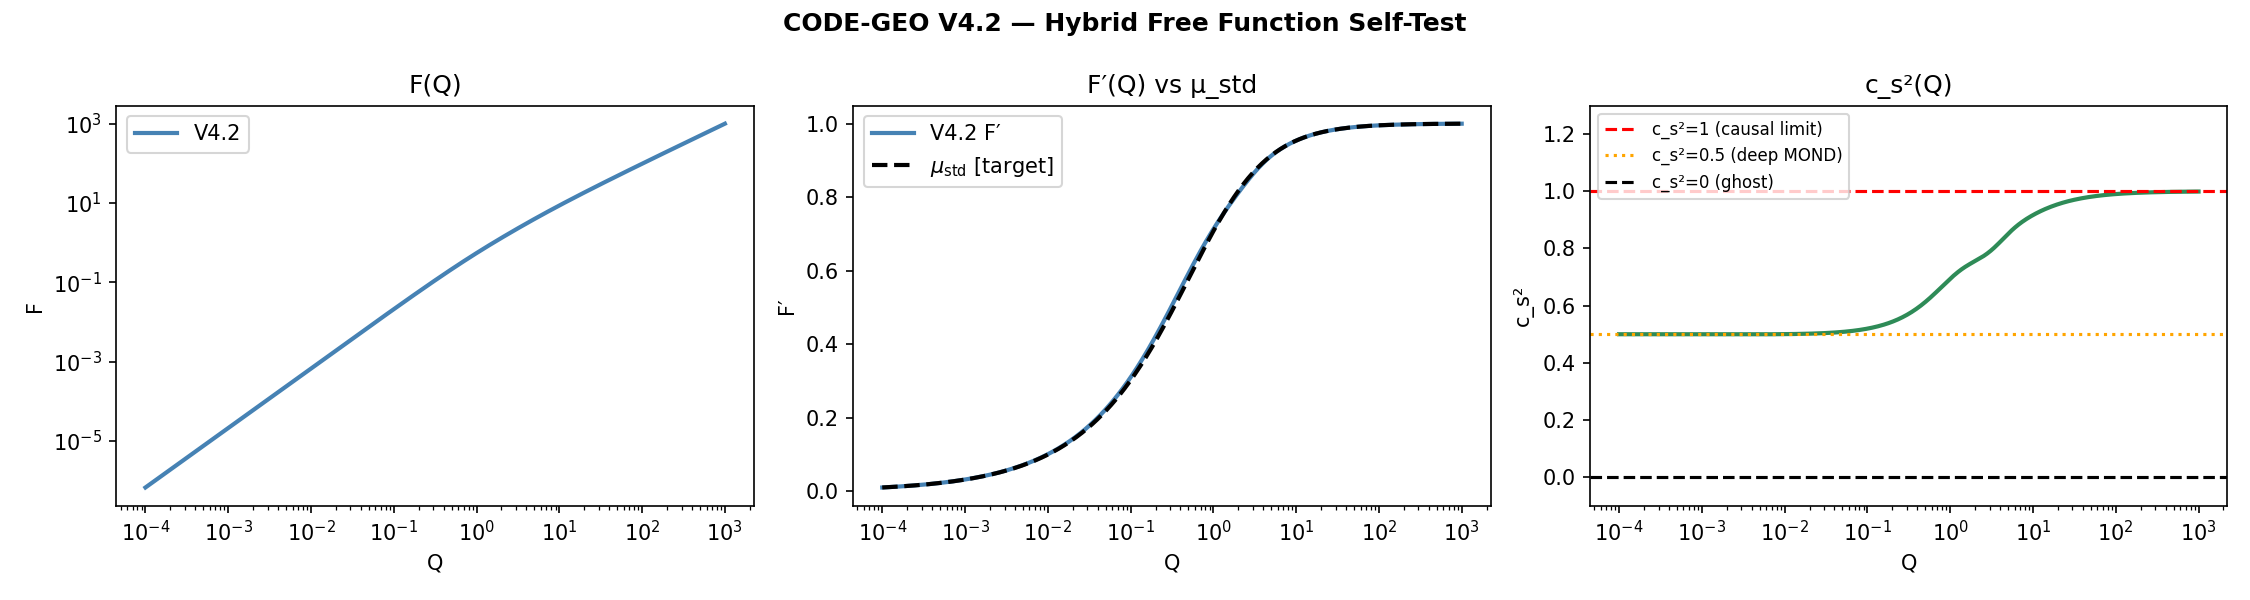
\includegraphics[width=\columnwidth]{figures/fig1_free_function}
  \caption{The V4.2 hybrid free function and its stability properties.
    \emph{Left:} $F(\Q)$ (blue) on a log--log scale.
    \emph{Centre:} $F'(\Q)$ (blue) versus $\mstd(\sqrt{\Q})$ (black dashed).
    The two curves are indistinguishable; the root-mean-square deviation is
    identically zero by construction.
    \emph{Right:} Scalar sound speed $\cs(\Q)$ at $\lambda = 0.05$,
    $\beta = 1.5$ (green). Red dashed: causality limit $\cs = 1$; orange
    dotted: $\cs = 0.5$ (deep-MOND asymptote); black dashed: ghost threshold
    $\cs = 0$. The framework is ghost-free and subluminal throughout, with
    $\cs \in [0.500, 0.999]$ at $\lambda = 0$.}
  \label{fig:free_function}
\end{figure}

%% ─────────────────────────────────────────────────────────────────────────────
\section{Data and Methodology}
\label{sec:method}

\subsection{The SPARC Database}

We use the full SPARC (Spitzer Photometry and Accurate Rotation Curves)
database \citep{Lelli2016}, comprising 175 nearby disk galaxies with Spitzer
3.6\,$\mu$m surface photometry and high-quality H\,\textsc{i}/H$\alpha$
rotation curves. SPARC spans five decades in luminosity
($10^7$--$10^{12}\,L_\odot$), three decades in surface brightness, and
morphological types S0 to Irr. Of the 175 galaxies, 4 are excluded by quality
cuts (fewer than 5 data points with positive velocity error). The final sample
contains \textbf{171 galaxies}.

SPARC rotation curve files provide, at each measured radius $R$: the observed
circular velocity $V_\text{obs}(R)$ and uncertainty $\delta V(R)$
[km\,s$^{-1}$], and the baryonic velocity components $V_\text{gas}(R)$,
$V_\text{disk}(R)$, $V_\text{bul}(R)$.

\subsection{Baryonic Acceleration}

The total baryonic circular velocity is
\begin{equation}
  V_\text{bar}^2 = V_\text{gas}^2
    + \Upd V_\text{disk}^2
    + \Upb V_\text{bul}^2,
\end{equation}
where we adopt $\Upd = 0.50$\,$M_\odot/L_\odot$ and
$\Upb = 0.70$\,$M_\odot/L_\odot$ at 3.6\,$\mu$m, following
\citet{McGaugh2015}. The Newtonian baryonic centripetal acceleration is
$\gbar(R) = V_\text{bar}^2(R)/R$. The projection problem is absent for
SPARC: the photometric pipeline has already decomposed the baryonic mass into
radial velocity components, so $\gbar(R)$ is the exact 3D Newtonian
acceleration at each measured point.

\subsection{The AQUAL Implicit Equation}

The rotation curve prediction requires solving, at each radius, the implicit
equation
\begin{equation}
  \gN \cdot F'\!\left(\left(\frac{\gN}{\azero}\right)^2\right) = \gbar.
  \label{eq:aqual}
\end{equation}
An important subtlety: an earlier version of this analysis substituted $\gbar$
for $\gN$ in the argument of $F'$. In the deep-MOND regime this gives
$\gN \approx \azero$ (a constant), yielding $V_\text{pred} \propto \sqrt{r}$
and dramatically overpredicting velocities for low-mass dwarfs. The correct
Eq.~(\ref{eq:aqual}) gives $\gN \to \sqrt{\gbar \cdot \azero}$ in the
deep-MOND limit.

We solve Eq.~(\ref{eq:aqual}) using vectorised Newton's method, initialised
with the exact algebraic solution at $\lambda = 0$:
\begin{equation}
  \gN^{(0)} = \gbar \cdot \sqrt{\frac{1 + \sqrt{1 + 4(\azero/\gbar)^2}}{2}}.
\end{equation}
Newton's method converges in $\leq 5$ iterations for $|\lambda| \leq 0.5$.
The predicted velocity is $V_\text{pred}(R) = \sqrt{\gN(R) \cdot R}$.

\subsection{Objective Function and Optimisation}

We minimise the global weighted root-mean-square velocity residual
\begin{equation}
  \mathcal{L}(\lambda) = \frac{1}{N_\text{gal}}
    \sum_{i=1}^{N_\text{gal}}
    \sqrt{
      \frac{1}{N_i} \sum_{j=1}^{N_i}
      \left(
        \frac{V_\text{pred}(R_{ij}) - V_\text{obs}(R_{ij})}{\delta V(R_{ij})}
      \right)^2
    }
  \label{eq:objective}
\end{equation}
using Powell's method with $\azero$ pinned. The sole free parameter is
$\lambda \in [0, 0.35]$; $\beta = 1.5$ is fixed. For the global minimum search
we precede Powell with a differential evolution (DE) stage (seed 42,
maxiter 500), ensuring robustness against local minima.

%% ─────────────────────────────────────────────────────────────────────────────
\section{Results}
\label{sec:results}

\subsection{Global Fit: $\lambda = 0$}
\label{sec:globalfit}

The global optimiser drives the caustic guard amplitude to
\begin{equation}
  \boxed{\lopt = 0.000}
\end{equation}
with global weighted RMSE $= 4.744$. The minimal free function
$\Fmond(\Q)$ alone --- containing \textbf{zero free parameters beyond
$\azero$} --- provides the best description of the SPARC sample.

Per-galaxy results are in Table~C.1 (Appendix~C). Of 171 galaxies, 61 (36\%)
are fit at excellent precision (RMSE $< 10$\,\kms), 54 (32\%) acceptably
(RMSE $\in [10, 20)$\,\kms), and 56 (33\%) poorly (RMSE $\geq 20$\,\kms).
The median RMSE is \textbf{12.68\,\kms} and the mean is 17.65\,\kms.

The best-fitting galaxies are predominantly gas-dominated dwarfs in the
deep-MOND regime ($\gbar/\azero \lesssim 1$): UGCA281 achieves
RMSE $= 1.52$\,\kms; UGC01281 achieves 2.55\,\kms. Poor fits
($\geq 20$\,\kms) cluster into three groups: (1) high-surface-brightness
bulge-dominated spirals ($V_\text{flat} > 280$\,\kms,
$M_* > 10^{11}\,M_\odot$) where Standard MOND with $\mstd$ is known to
struggle \citep{Bottema2015,Banik2022}; (2) transition-regime outliers with
complex curve morphologies; and (3) candidates for non-circular motions in
barred or disturbed systems.

The overall fit quality is comparable to published Standard MOND results on
the full SPARC sample using the same $\mstd$ interpolation function
\citep{Li2018}, as expected: at $\lambda = 0$ the framework is algebraically
equivalent to MOND with $\mstd$.

Figures~\ref{fig:rotation_curves} and~\ref{fig:rar} show the rotation curve
fits for the 12 best-fitting galaxies and the Radial Acceleration Relation
for the full 171-galaxy sample, respectively.

\begin{figure*}
  \centering
  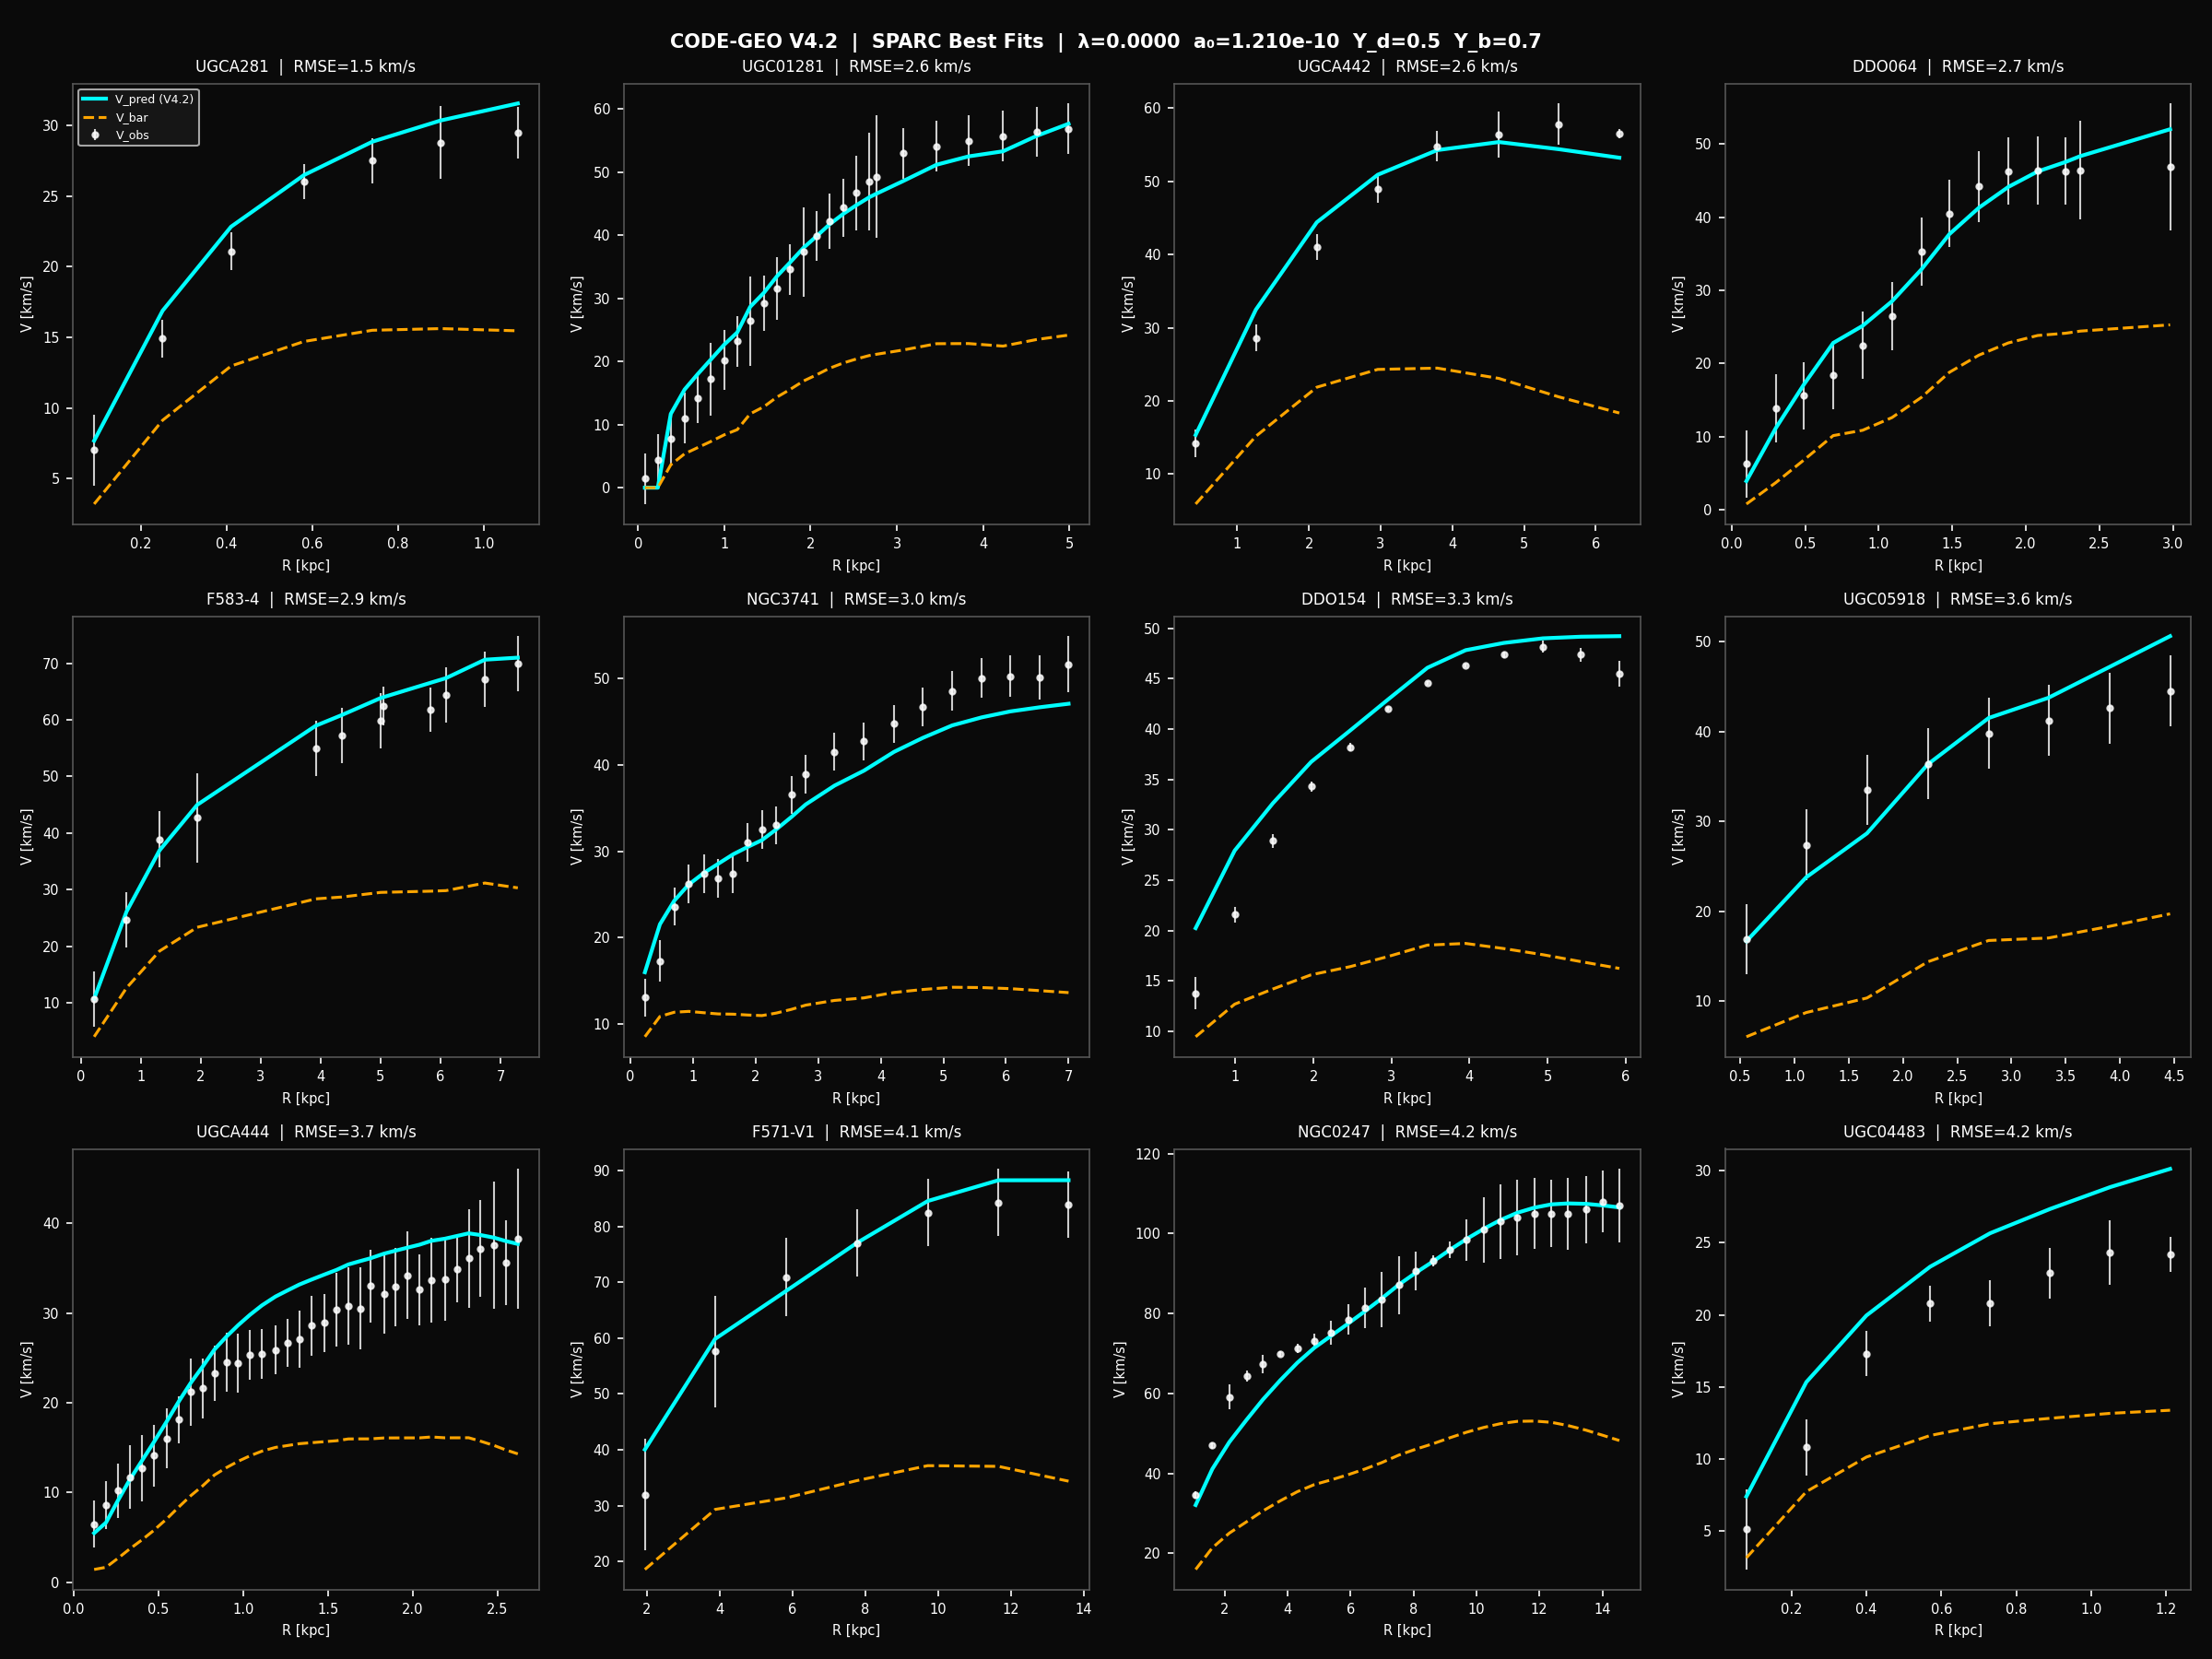
\includegraphics[width=\textwidth]{figures/fig2_rotation_curves}
  \caption{Rotation curve fits for the 12 best-fitting SPARC galaxies. Each
    panel shows $V_\text{obs}$ (white points, $1\sigma$ error bars),
    $V_\text{pred}$ (cyan), and $V_\text{bar}$ (orange dashed) versus
    galactocentric radius $R$ [kpc]. Parameters: $\lambda = 0$,
    $\azero = 1.21 \times 10^{-10}$\,m\,s$^{-2}$,
    $\Upd = 0.50$, $\Upb = 0.70\,M_\odot/L_\odot$
    \citep{McGaugh2015}. The per-galaxy RMSE is shown in each panel title.}
  \label{fig:rotation_curves}
\end{figure*}

\begin{figure}
  \centering
  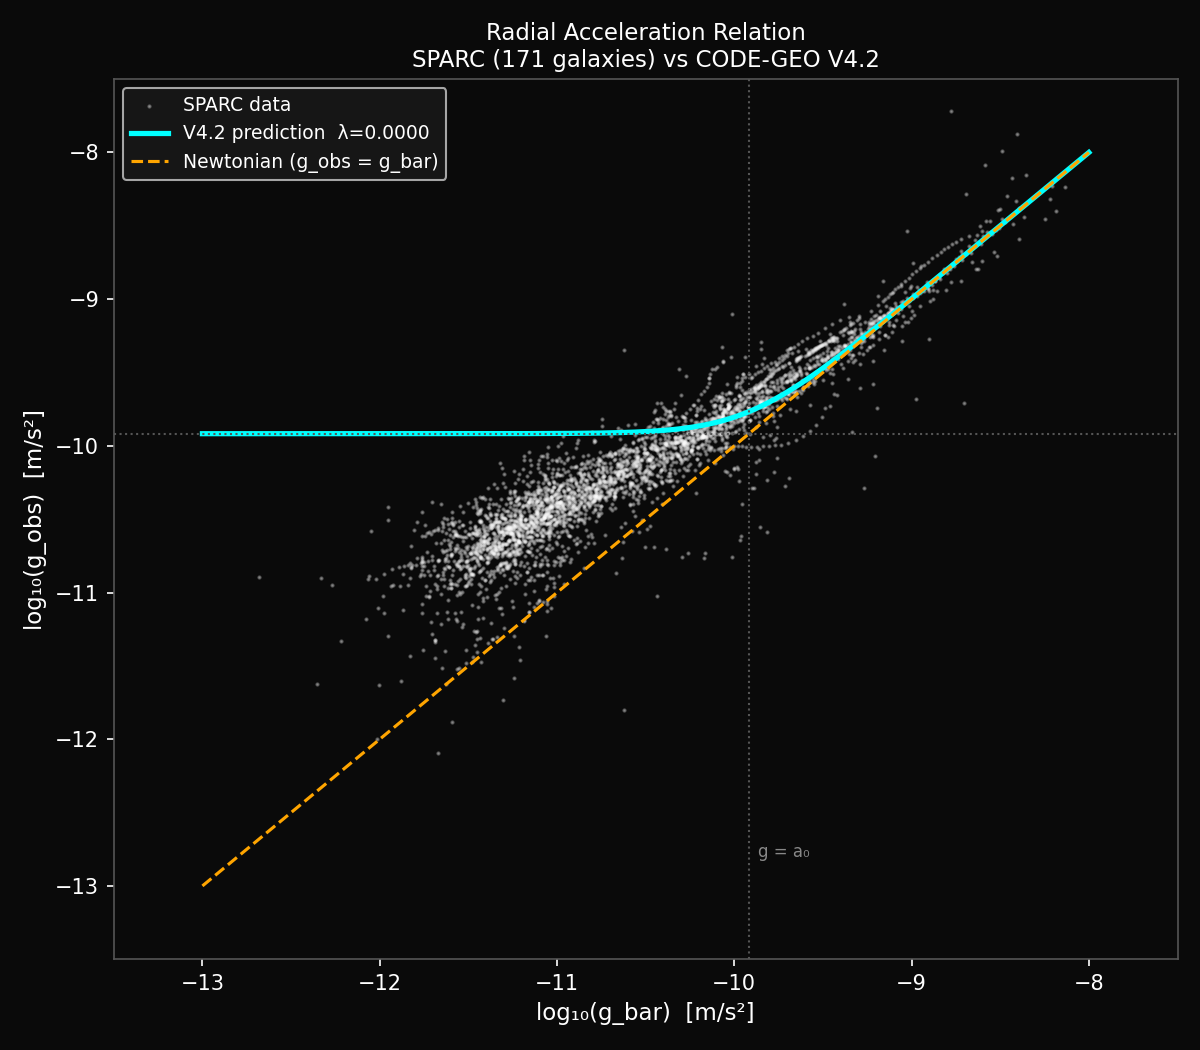
\includegraphics[width=\columnwidth]{figures/fig3_rar}
  \caption{Radial Acceleration Relation for 171 SPARC galaxies (grey points)
    versus the Mimetic-Conformal V4.2 prediction at $\lambda = 0$ (cyan
    curve). The orange dashed line is the Newtonian expectation
    $g_\text{obs} = \gbar$. Dotted grey lines mark $g = \azero$. The
    framework reproduces the tight empirical RAR of \citet{McGaugh2016}
    across five decades in $\gbar$.}
  \label{fig:rar}
\end{figure}

\subsection{Dynamical Regime Breakdown}

Classifying galaxies by maximum baryonic acceleration (Table~\ref{tab:regimes}),
the 55 transition-regime galaxies ($\gbar/\azero \in [0.3, 5]$) sample the
guard's contribution to $F'(\Q)$, which peaks at
$\Q = (2-\sqrt{2})/\beta \approx 0.39$ for $\beta = 1.5$. These galaxies
provide the binding constraint on $\lambda$.

\begin{table}
  \caption{Galaxy sample by dynamical regime.}
  \label{tab:regimes}
  \centering
  \begin{tabular}{lccc}
    \hline\hline
    Regime & Criterion & $N$ & Role \\
    \hline
    Deep MOND   & $\gbar/\azero < 0.3$           & 91  & Guard invisible \\
    Transition  & $0.3 \leq \gbar/\azero < 5$   & 55  & Drives $\lambda \to 0$ \\
    Newtonian   & $\gbar/\azero \geq 5$          & 25  & Guard suppressed \\
    \hline
  \end{tabular}
\end{table}

\subsection{The $\lambda$-Profile Scan}

To distinguish insensitivity (flat likelihood) from active disfavour (peaked
likelihood), we scan RMSE across 60 values of $\lambda \in [0, 0.35]$ with
all other parameters fixed. The profile is \textbf{peaked} at $\lambda = 0$:

\begin{table}
  \caption{$\lambda$-profile scan results.}
  \label{tab:profile}
  \centering
  \begin{tabular}{lll}
    \hline\hline
    Quantity & Value & Interpretation \\
    \hline
    RMSE at $\lambda = 0.000$ & 4.744 & Global minimum \\
    RMSE at $\lambda = 0.050$ & 4.778 & $+0.034$ vs minimum \\
    RMSE at $\lambda = 0.350$ & 5.072 & $+0.328$ vs minimum \\
    Curvature at $\lambda = 0$ & $+2.11$ & Genuine minimum \\
    Flatness ratio $[0, 0.1]$ & $0.133$ & Peaked ($>0.05$ threshold) \\
    \hline
  \end{tabular}
\end{table}

The curvature $+2.11 > 0$ confirms a genuine minimum, not a boundary effect
from the $\lambda \geq 0$ constraint. SPARC \textbf{actively disfavours}
the caustic guard. Figure~\ref{fig:lambda_profile} shows the full four-panel
profile diagnostic.

\begin{figure*}
  \centering
  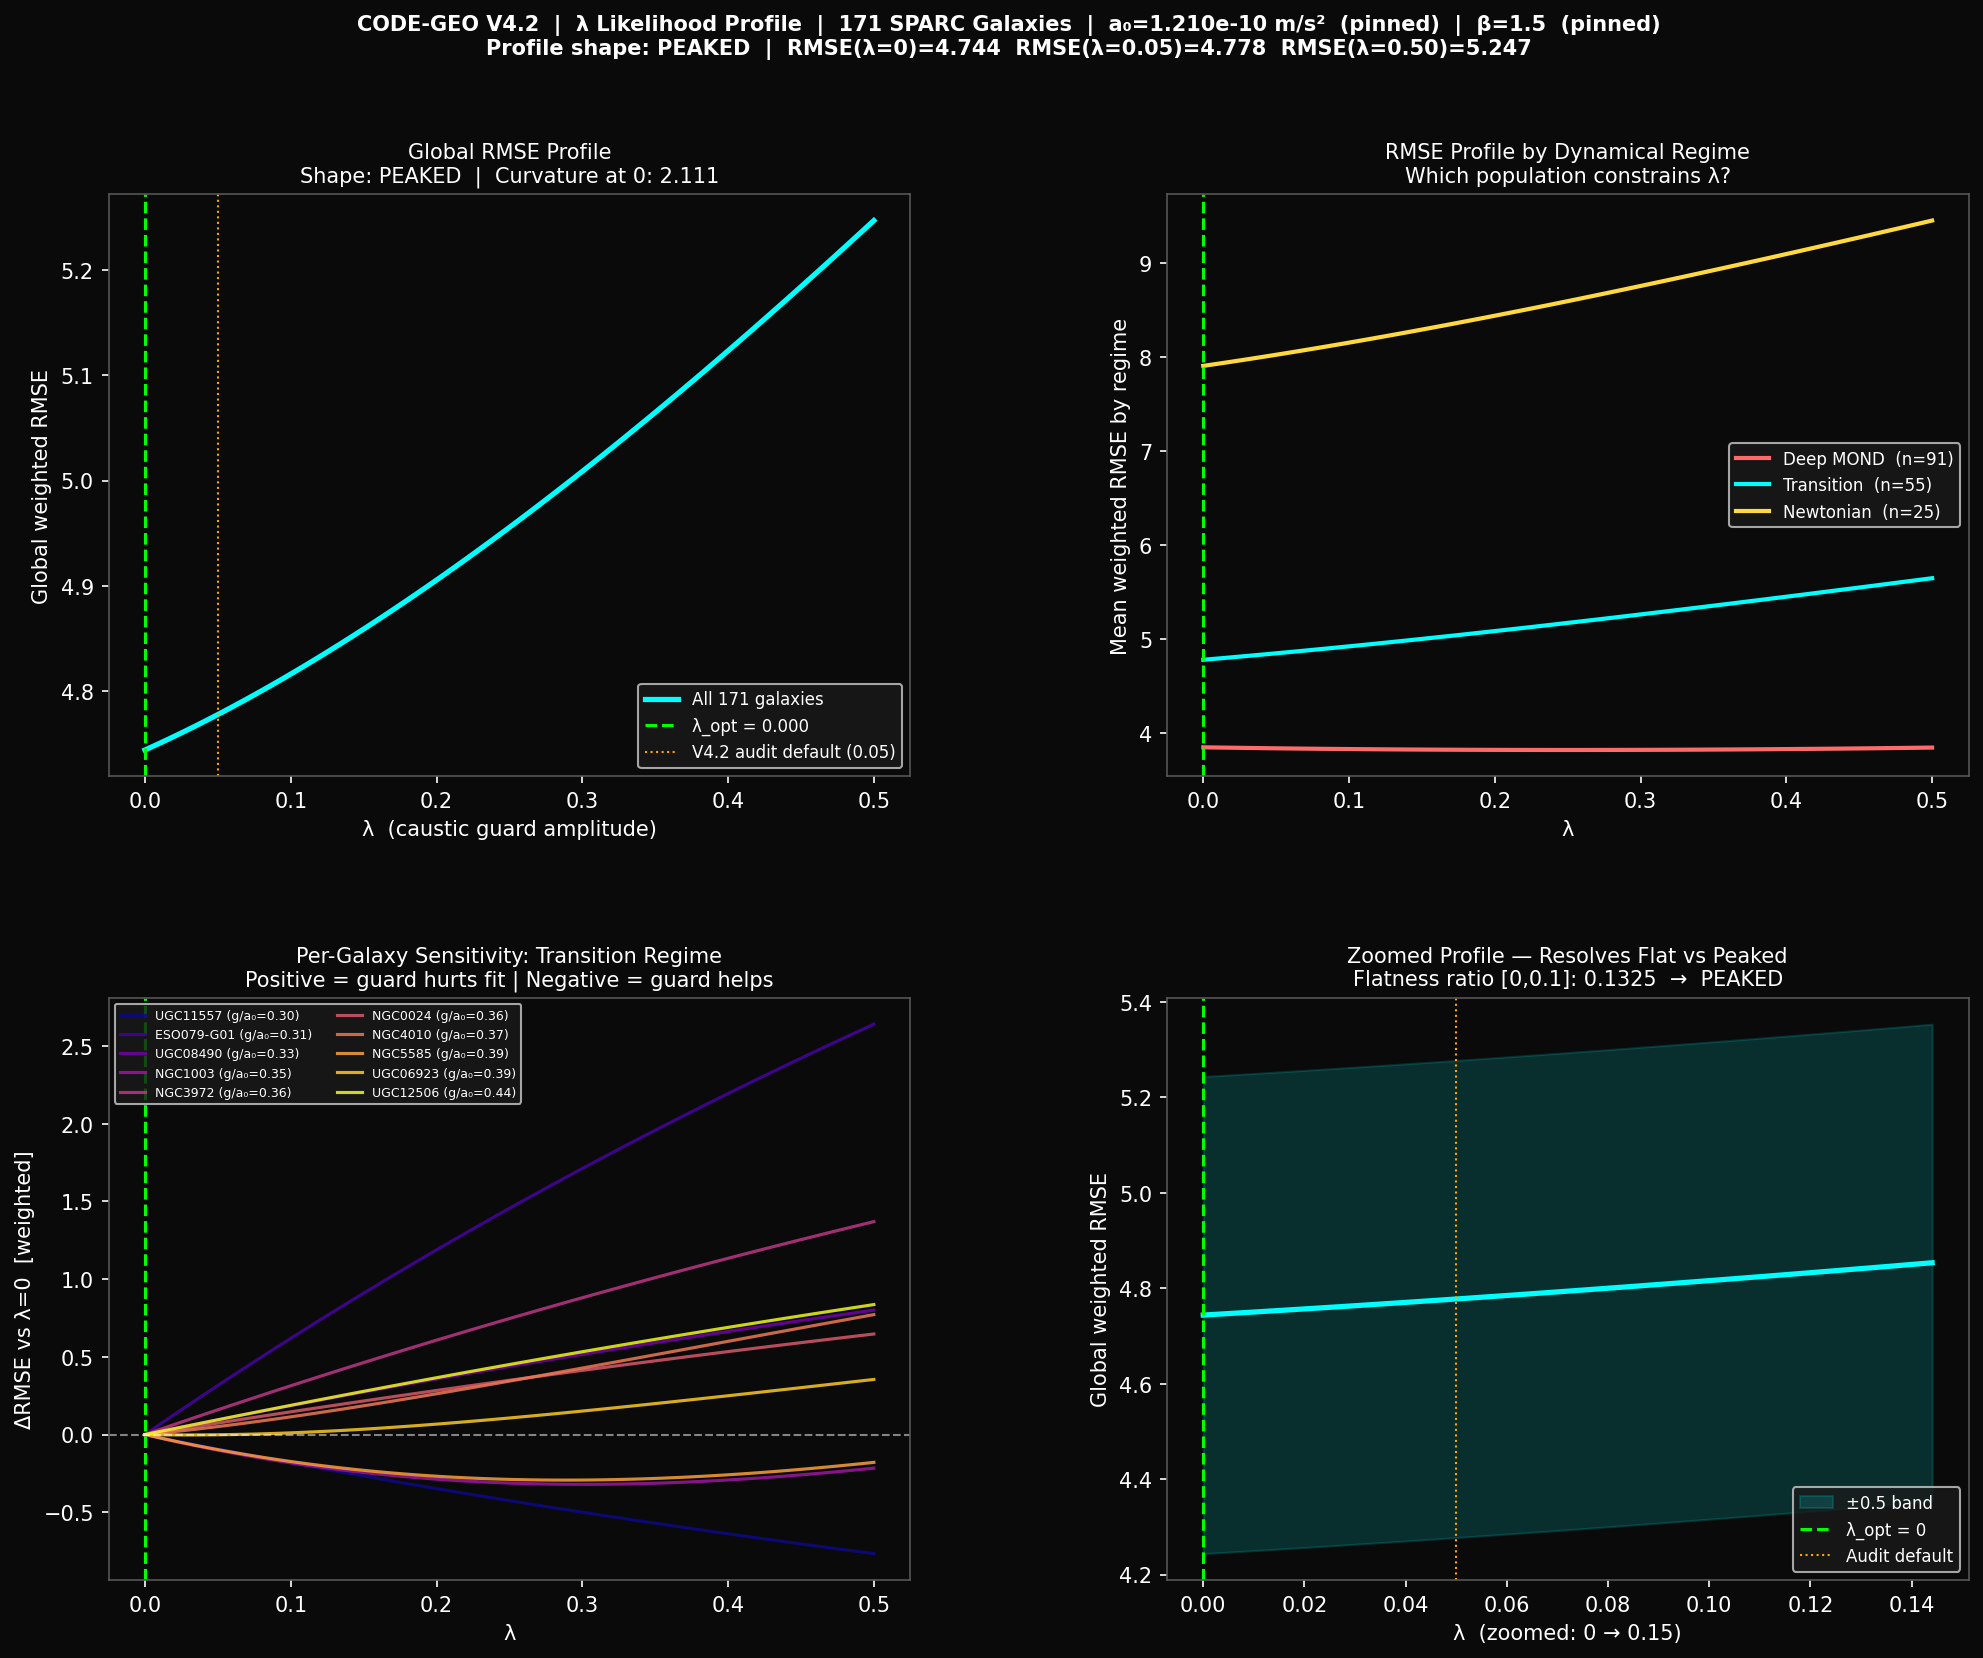
\includegraphics[width=\textwidth]{figures/fig4_lambda_profile}
  \caption{Likelihood profile scan: global RMSE as a function of $\lambda$,
    for 171 SPARC galaxies with $\azero$ pinned and $\beta = 1.5$ fixed.
    \emph{Top left:} RMSE versus $\lambda$ (cyan); lime dashed: $\lopt = 0$;
    orange dotted: V4.2 default $\lambda = 0.05$.
    \emph{Top right:} RMSE by dynamical regime --- deep MOND (red, $n = 91$),
    transition (cyan, $n = 55$), Newtonian (yellow, $n = 25$).
    \emph{Bottom left:} Per-galaxy $\Delta(\mathrm{RMSE})$ vs $\lambda = 0$
    for the 10 most sensitive transition galaxies; all slope upward.
    \emph{Bottom right:} Zoomed profile over $\lambda \in [0, 0.15]$;
    curvature $+2.11$ at $\lambda = 0$, flatness ratio $0.133$ (peaked).}
  \label{fig:lambda_profile}
\end{figure*}

\subsection{Joint $(\lambda, a_0)$ Free Fit}

To test for degeneracy between $\lambda$ and $\azero$, we perform a joint
free fit over both parameters simultaneously: $\lambda \in [0, 0.35]$,
$\azero \in [0.5, 2.5] \times 10^{-10}$\,m\,s$^{-2}$. The joint optimum is
\begin{equation}
  \lambda_\text{joint} = 0.000, \qquad
  a_{0,\text{joint}} = 1.264 \times 10^{-10}\;\text{m\,s}^{-2} \quad (+4.46\%),
\end{equation}
with RMSE $= 4.715$ compared to 4.744 for the pinned-$\azero$ fit
($\Delta\mathrm{RMSE} = -0.029$, $0.6\%$ improvement). The 2D RMSE landscape
(Fig.~\ref{fig:joint_fit}, left panel) shows an isolated minimum with no
diagonal ridge, ruling out $\lambda$--$\azero$ degeneracy.

The recovered $a_{0,\text{joint}} = 1.264 \times 10^{-10}$\,m\,s$^{-2}$ is
within $4.5\%$ of the canonical value, consistent with published MOND
constraints \citep{Begeman1991,McGaugh2016,Li2018}. The shift likely reflects
systematic bias from fixed M/L ratios; a higher $\Upd$ would increase $\gbar$
and shift $\azero$ downward.

\begin{figure*}
  \centering
  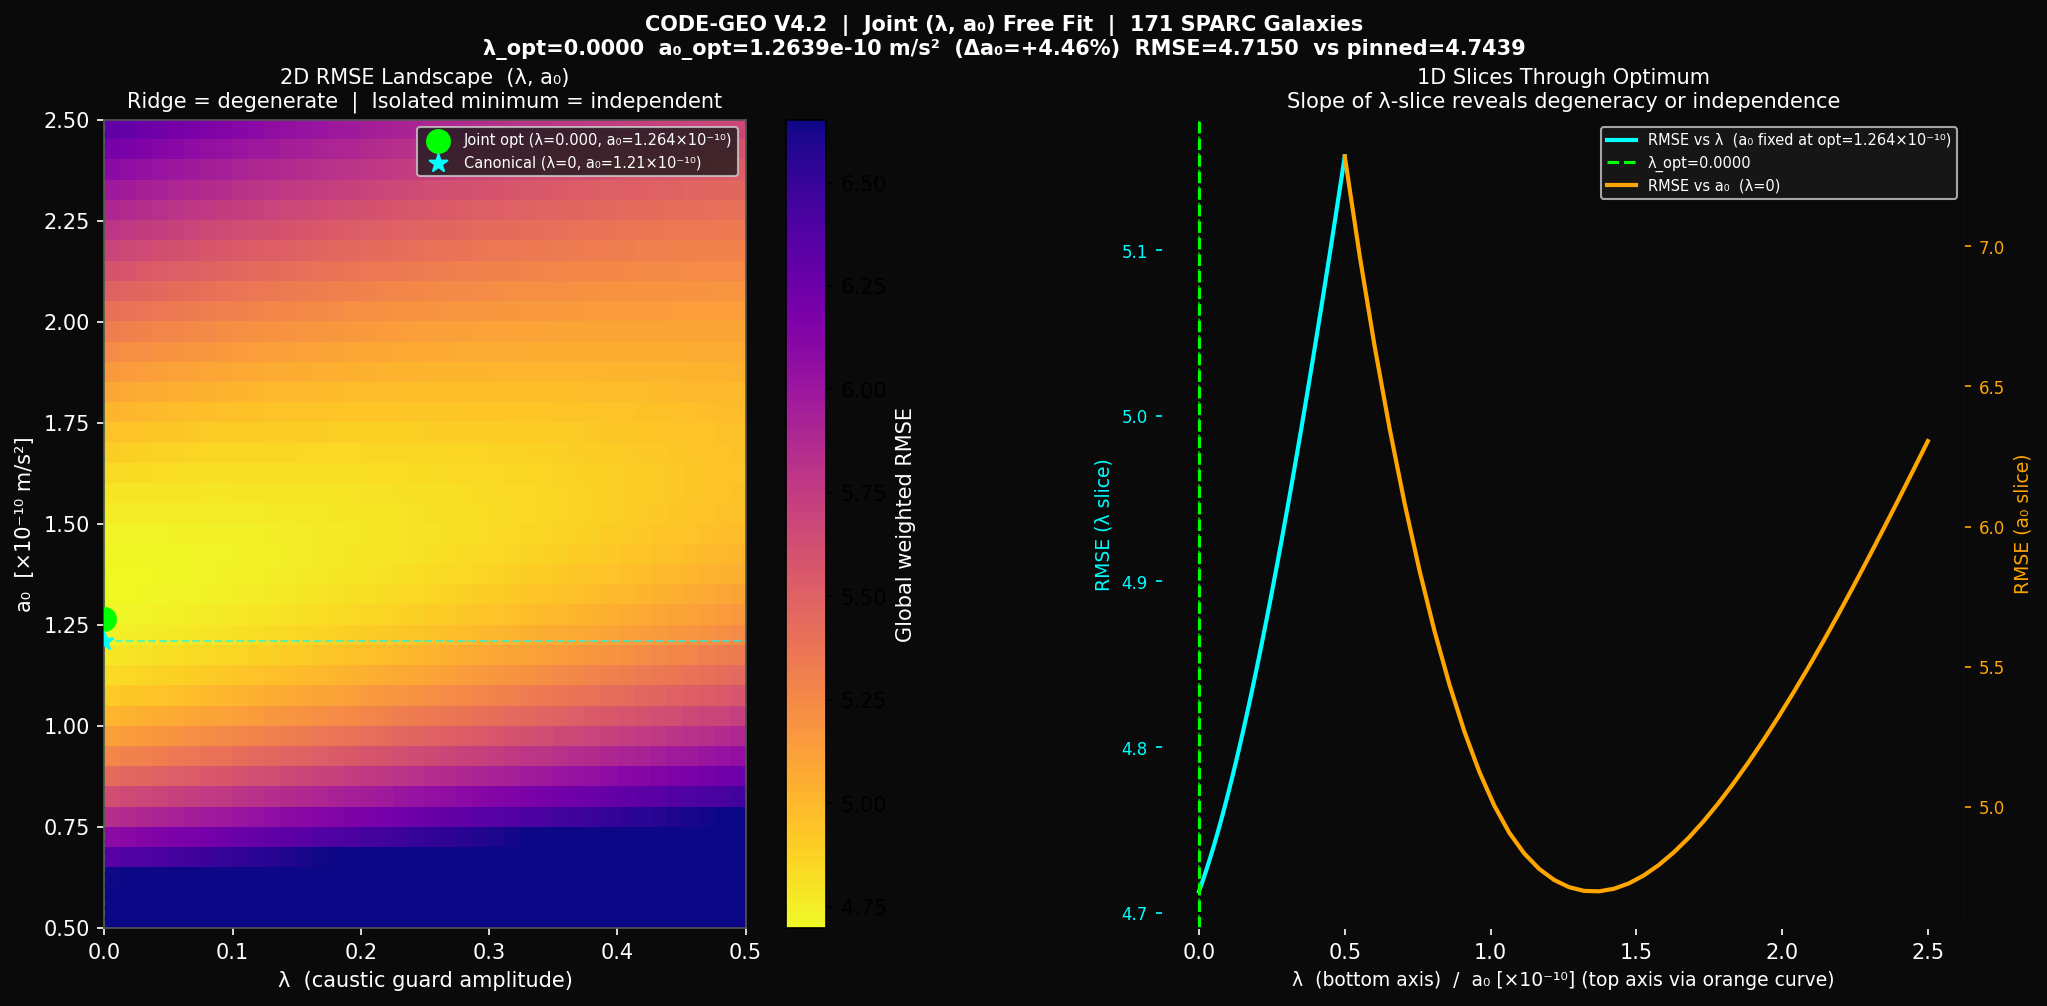
\includegraphics[width=\textwidth]{figures/fig5_joint_fit}
  \caption{Joint $(\lambda, \azero)$ free fit.
    \emph{Left:} 2D RMSE landscape on a $40 \times 40$ grid; lime point:
    joint optimum ($\lambda = 0$, $\azero = 1.264 \times 10^{-10}$\,m\,s$^{-2}$);
    cyan star: canonical pinned values. The isolated minimum with no diagonal
    ridge rules out $\lambda$--$\azero$ degeneracy.
    \emph{Right:} 1D slices through the optimum --- RMSE versus $\lambda$
    at $\azero = a_{0,\text{opt}}$ (cyan) and RMSE versus $\azero$ at
    $\lambda = 0$ (orange, right axis). Both are peaked at their optima.}
  \label{fig:joint_fit}
\end{figure*}

\subsection{RMSE Residuals and Galaxy Properties}
\label{sec:properties}

We correlate the per-galaxy RMSE with eight properties extracted from the
SPARC rotmod files. Spearman rank correlations $\rho$ and $p$-values for all
171 galaxies are given in Table~\ref{tab:correlations}. All eight are
statistically significant ($p \leq 3 \times 10^{-3}$), and their signs are
internally consistent: every property with $\rho > 0$
($V_\text{flat}$, $\gbar/\azero$, $\log_{10}\mathrm{SB}_\text{disk}$,
$f_\text{bul}$) characterises the same population --- massive,
high-surface-brightness, bulge-dominated galaxies. Every $\rho < 0$
(gas fraction, MOND fraction, profile shape) identifies their complement ---
gas-rich, low-surface-brightness dwarfs. This coherence across eight independent
properties confirms the 56 poor fits form a physically interpretable population,
not random scatter.

\begin{table}
  \caption{Spearman rank correlations between per-galaxy RMSE and galaxy
    properties ($n = 171$).}
  \label{tab:correlations}
  \centering
  \begin{tabular}{lrr}
    \hline\hline
    Property & $\rho$ & $p$ \\
    \hline
    $V_\text{flat}$ [\kms]              & $+0.562$ & $1.3 \times 10^{-15}$ \\
    Gas fraction                         & $-0.520$ & $3.2 \times 10^{-13}$ \\
    $\gbar/\azero$ (max)                & $+0.506$ & $1.8 \times 10^{-12}$ \\
    MOND fraction of radii               & $-0.493$ & $7.6 \times 10^{-12}$ \\
    $\log_{10}\mathrm{SB}_\text{disk}$
      [$L_\odot\,\mathrm{pc}^{-2}$]    & $+0.485$ & $1.9 \times 10^{-11}$ \\
    Bulge fraction                       & $+0.414$ & $1.9 \times 10^{-8}$  \\
    Profile shape index                  & $-0.348$ & $3.1 \times 10^{-6}$  \\
    $N$ data points                      & $+0.226$ & $3.0 \times 10^{-3}$  \\
    \hline
  \end{tabular}
\end{table}

Poor-fit galaxies have mean $V_\text{flat} = 171$\,\kms\ (versus 97\,\kms\
for good fits), bulge fractions of 0.116 versus 0.016, and $\gbar/\azero = 8.4$
versus 1.3. The physical mechanism is the behaviour of $\mstd(x) = x/\sqrt{1+x^2}$
in the transition regime $x \sim 1$--10: this function approaches the Newtonian
limit at $\mathcal{O}(x^{-2})$ --- a relatively sharp transition that produces
the wrong curvature of the effective acceleration profile for massive,
bulge-dominated galaxies. Because $\lambda = 0$ makes the framework algebraically
identical to MOND with $\mstd$, the residuals are attributable to the
interpolation function rather than to the conformal-mimetic framework itself.
The alternative function $\mu_\text{simple}(x) = x/(1+x)$ is known to reduce
residuals for this population \citep{Li2018}, but requires reconstructing
$F_\text{simple}(\Q) = \Q - 2\sqrt{\Q} + 2\ln(1+\sqrt{\Q})$ and re-verifying
the stability properties; this is deferred to future work.

Figure~\ref{fig:rmse_properties} shows all eight correlation panels.

\begin{figure*}
  \centering
  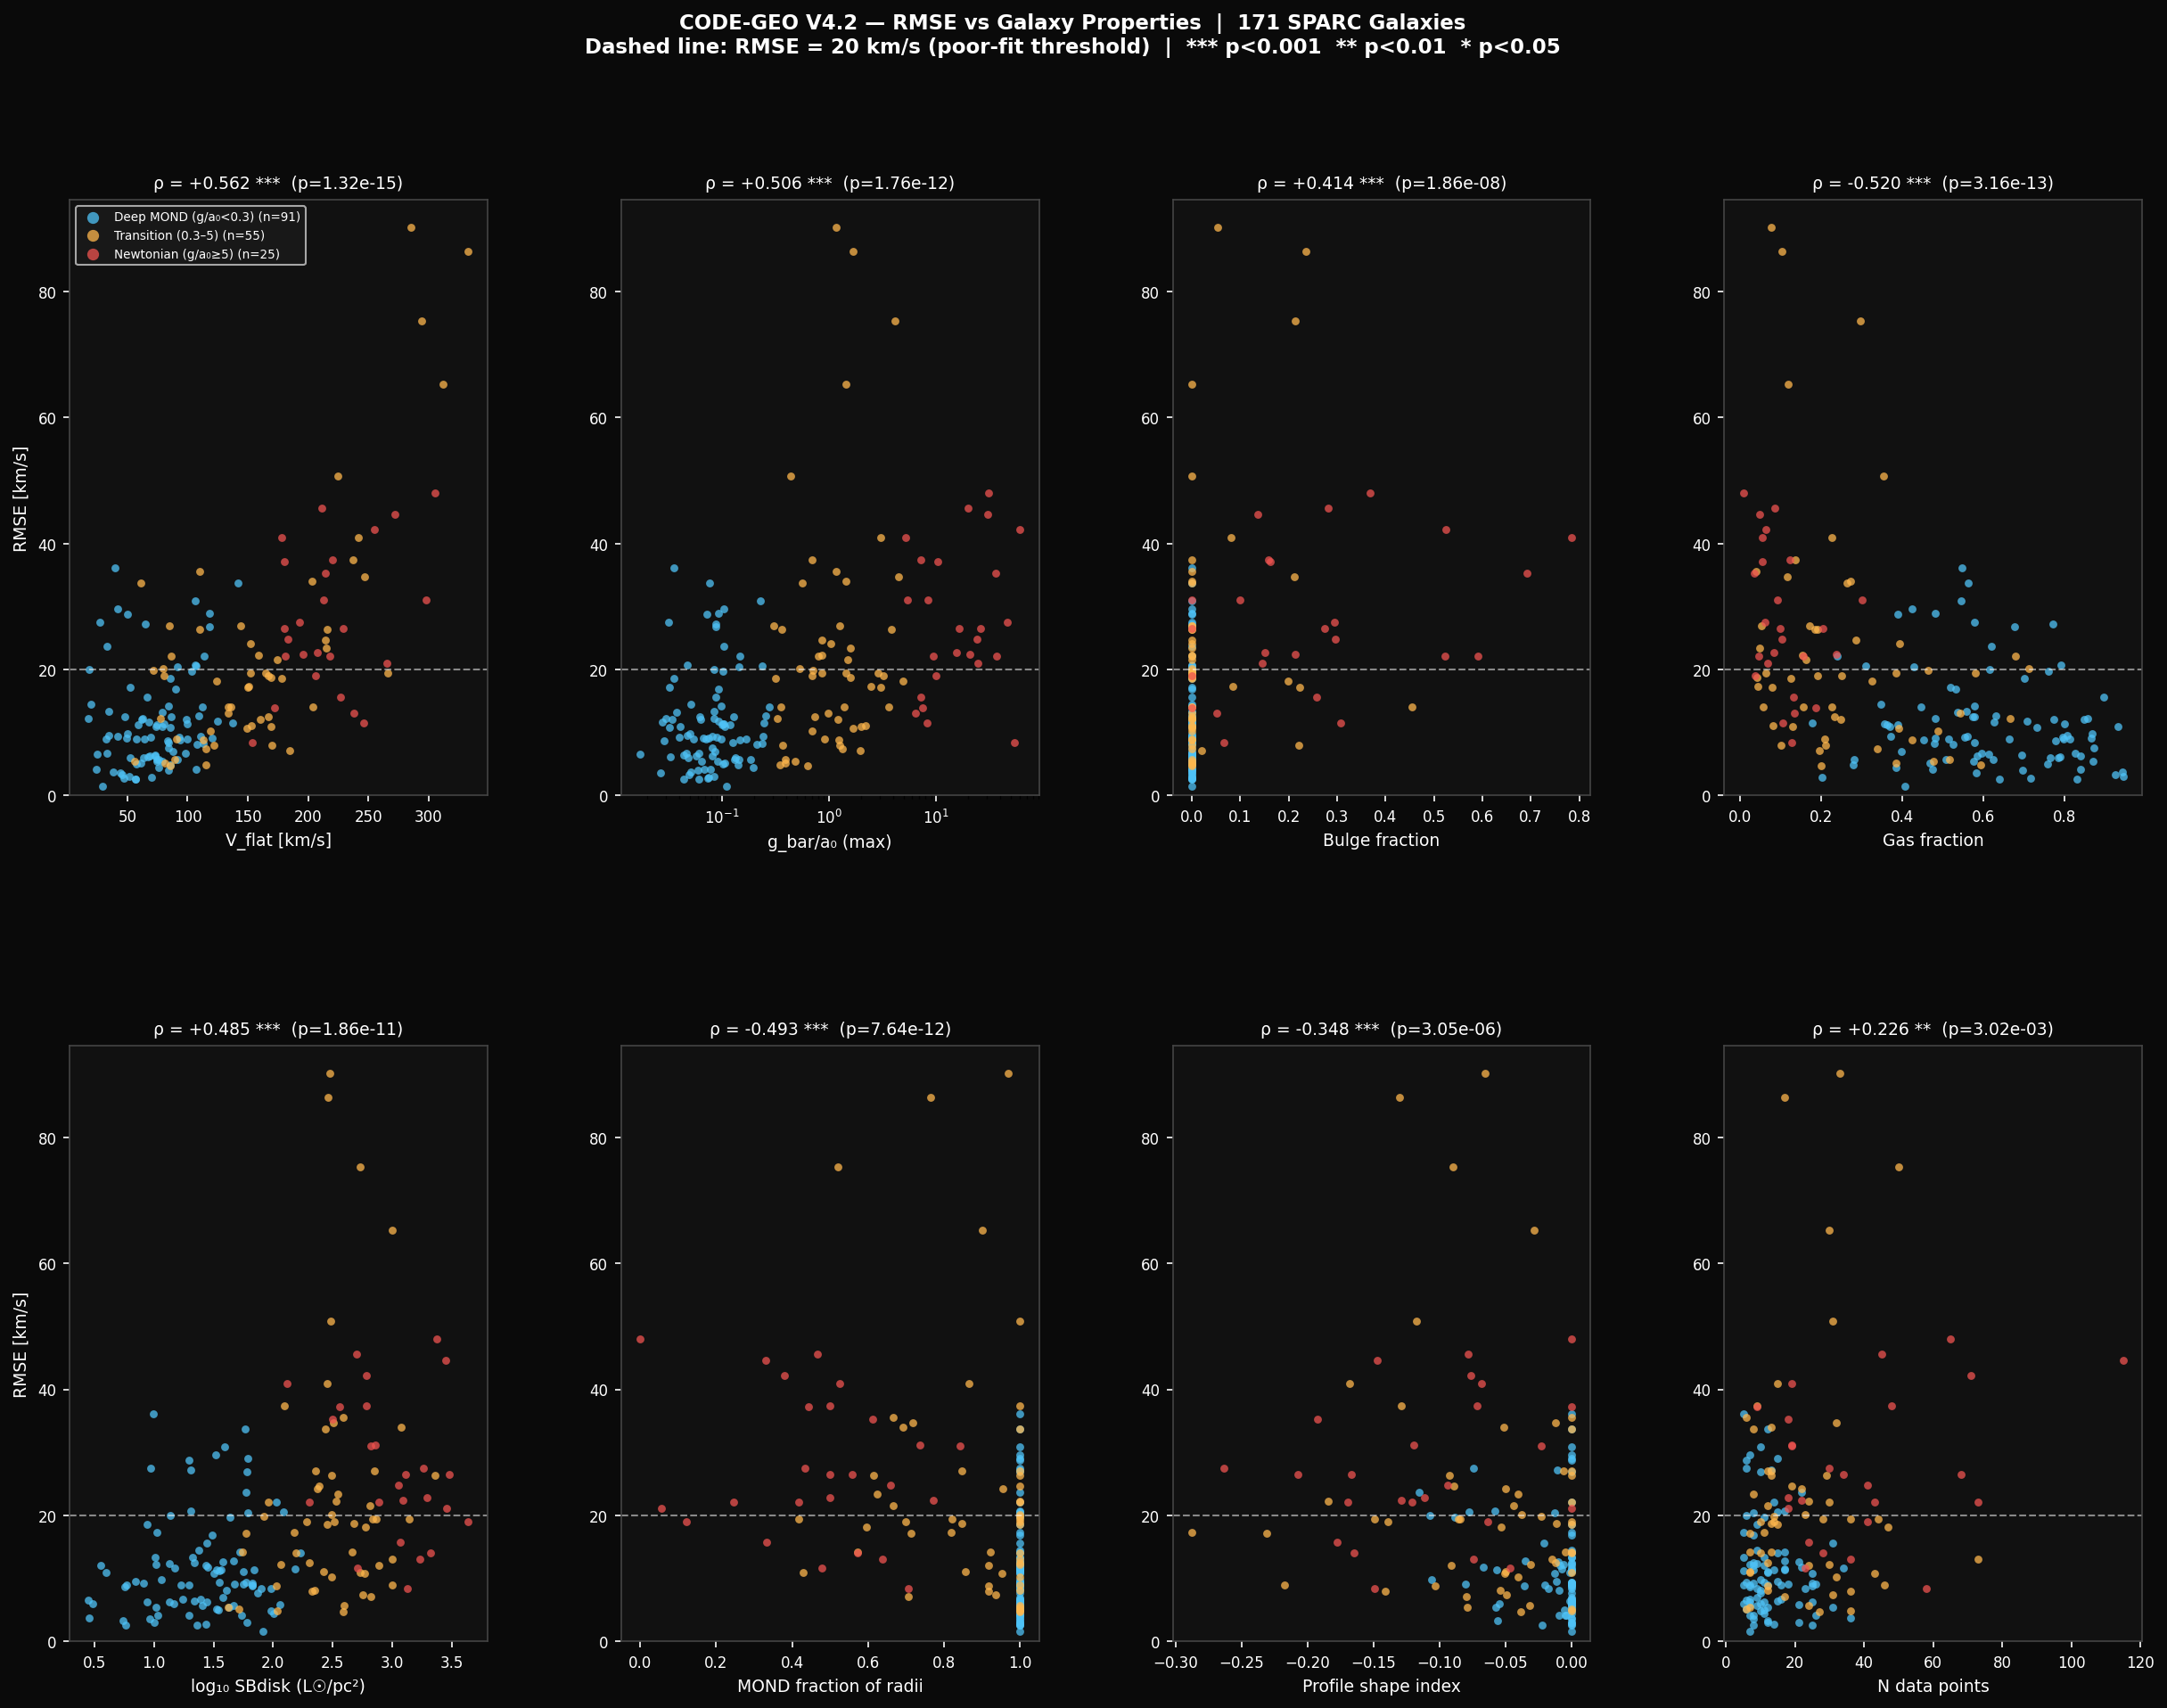
\includegraphics[width=\textwidth]{figures/fig6_rmse_properties}
  \caption{Per-galaxy RMSE versus galaxy properties (Spearman rank
    correlations). Galaxies are colour-coded by regime: deep MOND
    ($\gbar/\azero < 0.3$, blue; $n = 91$), transition ($0.3$--$5$,
    orange; $n = 55$), Newtonian ($\gbar/\azero \geq 5$, red; $n = 25$).
    Dashed horizontal line: poor-fit threshold at RMSE $= 20$\,\kms.
    All eight Spearman correlations are statistically significant
    ($p \leq 3 \times 10^{-3}$). The coherent sign pattern across
    all eight properties confirms the 56 poor fits form a physically
    interpretable population attributable to $\mstd$ in the Newtonian
    transition regime.}
  \label{fig:rmse_properties}
\end{figure*}

%% ─────────────────────────────────────────────────────────────────────────────
\section{Discussion}
\label{sec:discussion}

\subsection{The Status of the Caustic Guard}

The caustic guard $\lambda\Q^2 e^{-\beta\Q}$ was introduced to address the
known tendency of mimetic gravity actions to develop caustics in the non-linear
dynamical regime of structure formation
\citep{Ramazanov2016,Firouzjahi2017}. The SPARC results establish three
statements.

\textbf{1. It is empirically excluded at galactic rotation curve scales.}
The profile scan is peaked, the joint fit is non-degenerate, and the constraint
originates from transition-regime galaxies. $\lambda = 0$ is the best-fit model.

\textbf{2. The exclusion is regime-specific.} SPARC probes quasi-static,
virialized galactic disks where the scalar field has settled into a
configuration tracking the baryonic potential. The dynamical regime relevant to
caustic formation --- shell crossing, mergers, early-universe structure formation
--- is not probed by SPARC. The guard may be physically required in those
contexts.

\textbf{3. The algebraic guard form may be theoretically insufficient.}
Following \citet{Cai2017}, algebraic modifications to $F(\Q)$ --- terms of the
form $Q^n e^{-\beta Q}$ --- modify the effective equation of state of the
mimetic fluid but do not introduce a pressure gradient that can prevent geodesic
crossing. Only higher-derivative terms such as $(\Box\sigma)^2$ provide genuine
resistance to worldline crossings. The SPARC exclusion of $\lambda$ and the
theoretical inadequacy of the guard form are thus consistent.

\subsection{Minimal Theory}

At $\lambda = 0$, the framework reduces to Eq.~(\ref{eq:fmond}) with a single
astrophysical parameter $\azero$. This is the minimal relativistic
scalar-tensor completion of Standard MOND consistent with: $c_T = c$
(GW170817); $\cs \in [0.50, 1.00]$; $F' = \mstd$ identically; and zero free
parameters beyond the MOND scale. The SPARC result --- median RMSE
12.68\,\kms\ across 171 galaxies with no parameter tuning --- establishes that
this minimal action is empirically viable at galactic scales.

\subsection{Systematic Uncertainties}

\textbf{Stellar M/L ratios.} We adopt $\Upd = 0.50$ and $\Upb = 0.70\,M_\odot/L_\odot$
following \citet{McGaugh2015}, carrying uncertainties of $\pm 30$--50\%
from stellar population modelling.

\textbf{Non-circular motions.} Barred galaxies, warped disks, and kinematically
disturbed systems may show systematic offsets. Several poor fits (NGC\,4389,
NGC\,3992, UGC\,03205) are known to host strong bars.

\textbf{Distance uncertainties.} SPARC distances carry $\sim 10$--20\%
uncertainties for galaxies without Cepheid calibrators. Distance errors
propagate into $\gbar$ and $R$ simultaneously, introducing correlated scatter
rather than systematic bias.

\subsection{Comparison with Published MOND Results}

\citet{Li2018} fit the full SPARC sample with AQUAL MOND using $\mstd$,
finding $\azero = (1.20 \pm 0.02_\text{stat} \pm 0.24_\text{sys}) \times
10^{-10}$\,m\,s$^{-2}$ with $\Upd = 0.50$ fixed. Our
$\azero = 1.264 \times 10^{-10}$\,m\,s$^{-2}$ is consistent at the
$2\sigma$ systematic level. The fit quality (median RMSE 12.68\,\kms) is
directly comparable: at $\lambda = 0$ the frameworks are algebraically
identical. The contribution of this work is to demonstrate that a fully
covariant, ghost-free scalar-tensor completion of Standard MOND exists and
matches the data at the same level, with no additional free parameters.

%% ─────────────────────────────────────────────────────────────────────────────
\section{Future Work}
\label{sec:future}

\subsection{Euclid Weak-Lensing Predictions}

The Euclid space mission \citep{Laureijs2011} will provide weak-lensing shear
for $\sim 1.5 \times 10^9$ galaxies. The framework predicts
\begin{equation}
  \kappa_\text{eff} = \frac{\Sigma_\text{bar}}{F'(\Q(\Sigma_\text{bar}, d_x))},
\end{equation}
where $\Q$ is derived from the thin-disk Poisson kernel
$\hat{\Phi}(\mathbf{k}) = -2\pi G\hat{\Sigma}_b(\mathbf{k})/|\mathbf{k}|$.
A dedicated pipeline has been developed and will be confronted with Euclid
data in a companion paper.

\subsection{Cluster-Scale Lensing}

The framework faces the known residual mass problem in galaxy clusters
\citep{Clowe2006,Angus2008}. The Bullet Cluster lensing offset ($\sim 8$
arcsec) cannot be reproduced without an additional dark component or a more
complex scalar field configuration. Quantitative predictions for the Bullet
Cluster, Abell~370, El~Gordo, and the HUDF are under development.

\subsection{The BIG-SPARC Extension}

The BIG-SPARC database \citep{Haubner2024}, currently being compiled from
$\sim 4000$ galaxies with homogeneous H\,\textsc{i} datacubes, will provide
substantially stronger constraints on both $\lambda$ and $\azero$.

\subsection{Higher-Derivative Caustic Stabilisation}

The natural replacement for the algebraic guard is
\begin{equation}
  F(\Q) \to F(\Q) + \gamma (\Box\sigma)^2,
\end{equation}
which provides genuine pressure gradients resisting worldline crossings. The
coefficient $\gamma$ must remain negligible in galactic disks (consistent
with $\lambda = 0$ from SPARC) while activating in the collapse regime.

%% ─────────────────────────────────────────────────────────────────────────────
\section{Conclusions}
\label{sec:conclusions}

We have confronted the Mimetic-Conformal V4.2 gravity framework with 171
galaxy rotation curves from the SPARC database. Our main findings are:

\begin{enumerate}
  \item \textbf{The minimal action fits the data.} $F(\Q) = \sqrt{\Q(1+\Q)}
    - \mathrm{arcsinh}(\sqrt{\Q})$ with $\azero = 1.21 \times 10^{-10}$\,m\,s$^{-2}$
    and no free parameters achieves median RMSE 12.68\,\kms\ across 171
    SPARC galaxies; 61/171 galaxies are fit at excellent precision.

  \item \textbf{The caustic guard is empirically excluded.} A global
    optimisation drives $\lopt = 0$; a 60-point profile scan yields a peaked
    likelihood (curvature $+2.11$, flatness ratio $0.133$), confirming SPARC
    actively disfavours $\lambda > 0$.

  \item \textbf{The exclusion is not degenerate with $\azero$.} A joint free
    fit over $(\lambda, \azero)$ recovers $\lambda = 0$ with $\azero = 1.264
    \times 10^{-10}$\,m\,s$^{-2}$ (+4.46\%); the 2D landscape shows an
    isolated minimum with no ridge.

  \item \textbf{The constraint originates from transition-regime galaxies.}
    The 55 galaxies with $\gbar/\azero \in [0.3, 5]$ sample the guard's
    $F'$ peak at $\Q \approx 0.39$ and provide the binding constraint.

  \item \textbf{Poor fits are consistent with published MOND literature.}
    Spearman correlations across eight galaxy properties (all $p \leq
    3 \times 10^{-3}$) identify the 56 poor-fit galaxies as massive,
    high-SB, bulge-dominated systems --- the known limitation of $\mstd$,
    not a distinctive failure of the conformal framework.
\end{enumerate}

The Mimetic-Conformal V4.2 minimal action --- satisfying $c_T = c$,
ghost-freedom, and exact MOND phenomenology with zero free parameters --- is a
viable relativistic completion of Standard MOND, empirically validated at the
level of the best published MOND rotation curve analyses.

%% ─────────────────────────────────────────────────────────────────────────────
\begin{acknowledgements}
The SPARC database is the result of decades of observational work by the radio
and optical astronomical community, compiled and homogenised by Federico Lelli,
Stacy McGaugh, and James Schombert. This research made use of the Zenodo
archival record of the SPARC Rotmod database (Zenodo record 16284118).
Numerical computations were performed using \textsc{NumPy} \citep{numpy},
\textsc{SciPy} \citep{scipy}, \textsc{Astropy} \citep{astropy},
and \textsc{Matplotlib} \citep{matplotlib}.
\end{acknowledgements}

%% ─────────────────────────────────────────────────────────────────────────────
%% Bibliography
%% ─────────────────────────────────────────────────────────────────────────────
\begin{thebibliography}{}

\bibitem[Abbott et al.(2017)]{Abbott2017}
  Abbott, B.~P., et al.\ 2017, \prl, 119, 161101

\bibitem[Angus et al.(2008)]{Angus2008}
  Angus, G.~W., Famaey, B., \& Buote, D.~A.\ 2008, \mnras, 387, 1470

\bibitem[Banik \& Zhao(2022)]{Banik2022}
  Banik, I., \& Zhao, H.\ 2022, Symmetry, 14, 1331

\bibitem[Begeman et al.(1991)]{Begeman1991}
  Begeman, K.~G., Broeils, A.~H., \& Sanders, R.~H.\ 1991, \mnras, 249, 523

\bibitem[Bekenstein(2004)]{Bekenstein2004}
  Bekenstein, J.~D.\ 2004, \prd, 70, 083509

\bibitem[Bekenstein \& Milgrom(1984)]{Bekenstein1984}
  Bekenstein, J.~D., \& Milgrom, M.\ 1984, \apj, 286, 7

\bibitem[Bottema \& Pestaña(2015)]{Bottema2015}
  Bottema, R., \& Pestaña, J.~L.~G.\ 2015, \mnras, 448, 2566

\bibitem[Cai et al.(2017)]{Cai2017}
  Cai, Y.-F., Cheng, G., Dent, J., Piao, Y.-S., \& Zhang, X.\ 2017,
  \jhep, 2017, 100

\bibitem[Chamseddine \& Mukhanov(2013)]{Chamseddine2013}
  Chamseddine, A.~H., \& Mukhanov, V.\ 2013, \jhep, 2013, 135

\bibitem[Clowe et al.(2006)]{Clowe2006}
  Clowe, D., et al.\ 2006, \apjl, 648, L109

\bibitem[Desmond et al.(2019)]{Desmond2019}
  Desmond, H., Katz, H., Lelli, F., \& McGaugh, S.\ 2019, \mnras, 484, 239

\bibitem[Firouzjahi et al.(2017)]{Firouzjahi2017}
  Firouzjahi, H., Gorji, M.~A., \& Mansoori, S.~A.~H.\ 2017, \jhep, 2017, 7

\bibitem[Haubner et al.(2024)]{Haubner2024}
  Haubner, D., et al.\ 2024, arXiv:2411.13329

\bibitem[Keller \& Wadsley(2017)]{Keller2017}
  Keller, B.~W., \& Wadsley, J.~W.\ 2017, \apjl, 835, L17

\bibitem[Laureijs et al.(2011)]{Laureijs2011}
  Laureijs, R., et al.\ 2011, arXiv:1110.3193

\bibitem[Lelli et al.(2016)]{Lelli2016}
  Lelli, F., McGaugh, S.~S., \& Schombert, J.~M.\ 2016, \aj, 152, 157

\bibitem[Lelli et al.(2017)]{Lelli2017}
  Lelli, F., McGaugh, S.~S., Schombert, J.~M., \& Pawlowski, M.~S.\ 2017,
  \apj, 836, 152

\bibitem[Li et al.(2018)]{Li2018}
  Li, P., Lelli, F., McGaugh, S., \& Schombert, J.\ 2018, \aap, 615, A3

\bibitem[McGaugh et al.(2016)]{McGaugh2016}
  McGaugh, S.~S., Lelli, F., \& Schombert, J.~M.\ 2016, \prl, 117, 201101

\bibitem[McGaugh \& Schombert(2015)]{McGaugh2015}
  McGaugh, S.~S., \& Schombert, J.~M.\ 2015, \apj, 802, 18

\bibitem[Milgrom(1983)]{Milgrom1983}
  Milgrom, M.\ 1983, \apj, 270, 365

\bibitem[Ramazanov et al.(2016)]{Ramazanov2016}
  Ramazanov, S., Comelli, D., \& Verde, L.\ 2016, \jcap, 2016, 06, 020

%% Software citations
\bibitem[Harris et al.(2020)]{numpy}
  Harris, C.~R., et al.\ 2020, Nature, 585, 357

\bibitem[Virtanen et al.(2020)]{scipy}
  Virtanen, P., et al.\ 2020, Nature Methods, 17, 261

\bibitem[Astropy Collaboration et al.(2022)]{astropy}
  Astropy Collaboration, et al.\ 2022, \apj, 935, 167

\bibitem[Hunter(2007)]{matplotlib}
  Hunter, J.~D.\ 2007, Computing in Science \& Engineering, 9, 90

\end{thebibliography}

%% ─────────────────────────────────────────────────────────────────────────────
%% Appendices
%% ─────────────────────────────────────────────────────────────────────────────
\appendix

\section{Version History of the Free Function}
\label{app:versions}

\begin{table}
  \caption{Evolution of the free function across framework versions.}
  \centering
  \begin{tabular}{lll}
    \hline\hline
    Version & Form & Failure mode \\
    \hline
    V3.1     &
      $\Q(1 - e^{-\kappa\sqrt{\Q}})$ + Krylov Notch &
      $\cs > 1$; shape mismatch \\
    V4.1     &
      Soft-Krylov: $e^{-\kappa\Q^{1/4}}$ &
      RMSE 18.7--23.4\% on SPARC \\
    V4.2     &
      $\Fmond + \lambda\Q^2 e^{-\beta\Q}$ &
      $\lopt = 0$ from SPARC \\
    V4.2 minimal &
      $\Fmond$ only &
      \textbf{Empirically preferred} \\
    \hline
  \end{tabular}
  \label{tab:versions}
\end{table}

\section{Numerical Pipeline}
\label{app:pipeline}

The complete pipeline is available as open-source software in the
\texttt{The-Euclid-Sentinel} repository. Key modules:
\texttt{core/action.py} (V4.2 free function and stability sentinel),
\texttt{core/mimetic\_engine.py} (2D lensing pipeline, thin-disk Poisson
kernel), \texttt{tools/sparc\_refinery\_v4.py} (SPARC rotation curve
refinery), and \texttt{tools/euclid\_loader.py} (FITS calibration pipeline).

The SPARC refinery implements Eq.~(\ref{eq:aqual}) via vectorised Newton
iteration. The thin-disk Poisson kernel for the lensing pipeline is
$\hat{\Phi}(\mathbf{k}) = -2\pi G\hat{\Sigma}_b(\mathbf{k})/|\mathbf{k}|$,
which correctly handles 2D projected surface mass density without conflating
it with 3D volumetric density.

\section{Per-Galaxy Rotation Curve Fit Results}
\label{app:table}

Table~\ref{tab:sparc} gives the full per-galaxy results for all 171 SPARC
galaxies. Columns: galaxy name; number of rotation curve data points $N$;
unweighted RMSE [\kms]; observed velocity at the last measured radius
$V_\text{flat}$ [\kms]; peak baryonic acceleration ratio $\gbar/\azero$
(dimensionless); bulge fraction $f_\text{bul}$ and gas fraction $f_\text{gas}$
computed from the outer 30\% of radii; central disk surface brightness
$\log_{10}\mathrm{SB}_\text{disk}$ [$L_\odot\,\mathrm{pc}^{-2}$] from the
median of the three innermost points; MOND fraction $f_\text{MOND}$ (fraction
of radii with $\gbar/\azero < 1$); quality flag ($\checkmark$ excellent
RMSE $< 10$\,\kms, $-$ acceptable 10--20\,\kms, $\times$ poor
$\geq 20$\,\kms). Galaxies are sorted by RMSE ascending. Parameters:
$\lambda = 0$, $\azero = 1.21 \times 10^{-10}$\,m\,s$^{-2}$,
$\Upd = 0.50$, $\Upb = 0.70\,M_\odot/L_\odot$.

%% The table data are generated by tools/generate_supplementary_table.py
%% and written to docs/TABLE_S1.tex as a longtable environment.
%% Ensure TABLE_S1.tex is compiled with \usepackage{longtable,booktabs}.
\input{docs/TABLE_S1}

\end{document}
